%
%-------------------------------------------------------------------------------
\clearpage\newpage
\section{PSHA disaggregation}
\label{sec:disaggregation}
%
Seismic hazard disaggregation - or deaggregation - 
\citep{mcguire1995,bazzurro1999} is a procedure aimed at identifying the 
contributions to a particular level of hazard at specific site -
produced by different combinations of basic variables - such as magnitude
and rupture-site distance - characterizing either the ruptures in the 
\gls{acr:erf} or the selected ground motion models.
%
Two are the main typologies of disaggregation currently adopted in PSHA 
studies (see for example \citet{petersen2008}): the m-r-$\epsilon$ 
disaggregation and the geographic disaggregation. 
%
Conceptually there are no differences between them; 
simply, in the geographic disaggregation the source-to-rupture 
distance is replaced by the position of the point used to calculate
the distance to the site.

Figure \ref{fig:mde_disaggregation} shows a 3-D plot representing the 
contribution to hazard provided by distinct discrete combinations of 
magnitude, distance and $\epsilon$. The usual information that can be
extracted from this plot is the dominant m-r couple \citep[for a 
discussion on this topic see][]{bazzurro1999}, that is the couple of 
parameters giving the highest contribution to the hazard disaggregated 
(i.e. the highest conditional exceedance probability). 
%
%
% . . . . . . . . . . . . . . . . . . . . . . . . . . . . . . . . . . . > Figure
\begin{figure}[!hb]
\centering
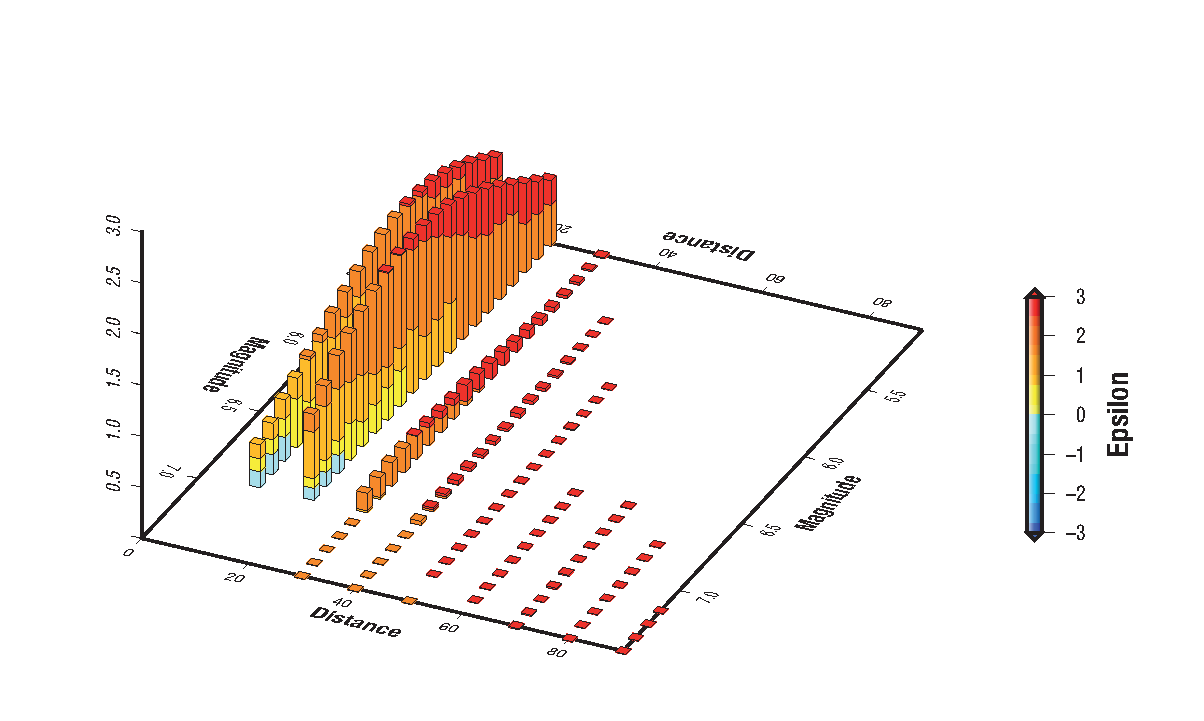
\includegraphics[width=15cm]{./Figures/Part_Hazard/disaggregation_mre.eps}
\caption{Example of the results provided by a magnitude-distance-$\epsilon$ 
disaggregation analysis.}
\label{fig:mde_disaggregation}
\end{figure}
% . . . . . . . . . . . . . . . . . . . . . . . . . . . . . . . . . . . < Figure
%

In \gls{acr:oq} we introduced a number of alternative disaggregation 
typologies that should help the modeller in better understanding the 
PSHA models and controlling the results provided for specific sites.
% 
In particular, we added the tectonic region and the seismic source type 
to the classical disaggregation variables (i.e. magnitude, distance and
epsilon); this way it will be possible to clearly identify the 
contributions to hazard coming from a several different combinations 
of variables and source and/or ground motion model attributes.
%
Indeed, the disaggregation methodologies implemented in \gls{acr:oq} is 
flexible enough to provide the disaggregation type according to the 
modeller's needs.
% 
\gls{acr:oq} supports disaggregation based on the classical PSHA 
methodology as well as on the event based methodology one. In the 
following sections we describe the details of the approaches
implemented.
%
%- - - - - - - - - - - - - - - - - - - - - - - - - - - - - - - - - - - - - - - -
\subsection{Disaggregation methodology}
From a calculation point of view, disaggregation simply consists 
firstly on systematically collecting the contributions (i.e. conditional 
probabilities of exceedance) to a selected value of hazard into a 
multidimensional matrix (called \gls{disaggregationmatrix}) and secondly 
to appropriately combine these contributions according to user 
instructions.
Usually a fraction of the ruptures included 
in an \gls{acr:erf} located at close distance to the reference site
provides the main contributions to the disaggregated hazard (see also 
Figure \ref{fig:mde_disaggregation}).

The \gls{disaggregationmatrix} used in \gls{acr:oq} contains the
following axes: magnitude (index i), longitude (index j), latitude 
(index k), source (index s) and epsilon (index l).
%
For each rupture the longitude and latitude coordinates corresponds 
to the point on the rupture used to calculate the source-site distance.
%
%. . . . . . . . . . . . . . . . . . . . . . . . . . . . . . . . . . . . . . . .
\subsubsection{Classical PSHA: examples of application of the 
disaggregation methodology}
%
In case of the classical PSHA methodology, the cumulation of 
contributions in the \gls{disaggregationmatrix} is based on a 
somewhat modified version of Equation \ref{eq:prob_y_ex_one_rup}.
This equation distinctly accounts for inputs to the probability of 
exceedance of $y$ coming from different $\epsilon$ intervals.
%
\begin{equation}
P(GM \geq y|t,rup_{src},\epsilon,site) = 
	P(rup_{src}|t)\,
	P(GM\geq y|rup_{src},\epsilon,site)
\label{eq:prob_y_ex_one_rup_eps}
\end{equation}
%
Equation \ref{eq:prob_y_ex_one_rup_eps} is used recursively to 
calculate (and successively store in the appropriate cell) the 
contribution coming from all the ruptures included in 
\gls{acr:erf}. 
%
%
\paragraph{Disaggregation in terms of tectonic region}
The disaggregation in terms of tectonic region is probably one of 
the simplest disaggregation from a conceptual point of view. 
%
It consists on cumulating in the disaggregation matrix the probabilities 
of exceedance computed in the innermost summation contained in the 
equation below:
\begin{multline}
P(GM \geq y|t,site) = \\
	1-\prod\limits_{\forall\,src\,\text{in}\,ERF}^{}  
	\left\{
		1-\sum\limits_{\forall\,rup\,\text{in}\,src}^{}
		\biggl[ 
			1-\sum\limits_{\forall\,\epsilon}^{} 
			P(GM \geq y|t,rup_{src},\epsilon,site)
		\biggr]
	\right\}
\label{eq:disaggregation_kernel}
\end{multline}
%
Successively, the calculations of the conditioned probabilities of 
exceedance for each tectonic region are computed using two nested
loops: the first for the tectonic regions defined in the PSHA the 
second for the seismic sources belonging to a given \gls{tectonicregion}. 
%
%
\paragraph{Disaggregation in terms of magnitude, distance and epsilon}
The magnitude-distance-$\epsilon$ disaggregation is, probably, the 
disaggregation typology most frequently adopted. 
%
%. . . . . . . . . . . . . . . . . . . . . . . . . . . . . . . . . . . . . . . .
\subsubsection{Event based PSHA: examples of application of the 
disaggregation methodology}
%
In case of the event-based PSHA methodology the disaggregation consist 
on the cumulation of the events with specific characteristics. 
